\chapter{Dimensionality reduction}
\section*{The Curse of Dimensionality}

%\subsection*{Introduction and Motivation}

The curse of dimensionality refers to various phenomena that arise when analyzing data in high-dimensional spaces. One of the most fundamental manifestations is that data becomes increasingly sparse as the number of dimensions grows, requiring exponentially more data points to maintain the same level of coverage.

To understand this phenomenon quantitatively, we analyze how many data points are needed to adequately cover a region of space as the dimensionality increases.

Consider a $D$-dimensional unit hypercube $[0,1]^D$, where each coordinate ranges from 0 to 1. This serves as our feature space, which can represent normalized features in a machine learning problem. The total volume of this hypercube is 1, regardless of dimension.

\subsection*{Grid-Based Analysis: Building Intuition}

\begin{description}
\item[One Dimension ($D=1$)] In one dimension, suppose we place points on a regular grid with spacing $l<1$ between consecutive points. Then, to cover the unit interval $[0,1]$, we need approximately $\frac{1}{l}$ points.% and if we want to cover only a fraction $p$ of the interval (say $p=0.5$), we need $\frac{p}{\epsilon} = \frac{0.5}{0.1} = 5$ points. The number of points scales linearly with $1/\epsilon$.

\item[Two Dimensions ($D=2$)] In two dimensions, we create a 2D grid with spacing $l$ along each axis. Along each dimension, we have $\frac{1}{l}$ points. The number of points needed to fill the unit square is clearly $\left(\frac{1}{l}\right)^2$.%, and to cover a fraction $p$ of the area, we need to fill a square of side length $\sqrt{p}$, requiring approximately $\left(\frac{\sqrt{p}}{\epsilon}\right)^2 = \frac{p}{\epsilon^2}$ points. The number of points scales quadratically with $1/\epsilon$—we need 100 times more points to reduce spacing by a factor of 10.

\item[$D$ Dimensions] Extending to $D$ dimensions, we observe that with spacing $l$ along each dimension, the total number of grid points needed to fill the entire unit hypercube is
$\left(\frac{1}{l}\right)^D
$
the number of points grows exponentially with dimension $D$.
\end{description}

Suppose each data point can only provide information about a fixed neighborhood of radius $r<1$.

Then the volume each point can cover is:
$$
\hat V(r) = \frac{\pi^{\frac{D}{2}}}{\Gamma(\frac{D}{2}+1)}r^D\sim r^D
$$

The total fraction of volume covered by $n$ points is at most (no intersection between volumes covered by different points)
$$
V = n \hat V \sim n  r^D
$$

Assuming now $V$ is fixed, solving for $n$ we get
$$
n \sim Vr^{-D}
$$

This is the exponential curse: to maintain fixed resolution $r$, you need $n \propto r^{-D}$ points to cover the space. The number of required points grows exponentially with dimension $D$.
\paragraph{Implications for Machine Learning}

This exponential growth has several critical consequences:

\begin{enumerate}
    \item \textbf{Data sparsity}: In high dimensions, available data becomes exponentially sparse. Even with millions of training examples, most of the input space remains unexplored and empty.
    
    \item \textbf{Sample complexity}: Learning algorithms that rely on local neighborhoods (like $k$-nearest neighbors) or that need to estimate densities become unreliable, as neighbors are exponentially far apart.
    
%    \item \textbf{Overfitting}: With sparse data in high dimensions, models can easily fit noise rather than true patterns, as there are exponentially many degrees of freedom but relatively few constraints from data.
\end{enumerate}

A different phenomenon occuring as the dimensionality $D$ increases is  \alert{distance concentration}: in high dimensions, the distance between any point and its nearest neighbor approaches the distance to its farthest neighbor. Specifically, for i.i.d. random points:
    $$
    \lim_{D \to \infty} \frac{\text{dist}_{max} - \text{dist}_{min}}{\text{dist}_{min}} \to 0
    $$
    This makes distance-based methods increasingly meaningless.


%\paragraph{Why This Matters for Machine Learning}

The curse of dimensionality provides strong motivation for dimensionality reduction in machine learning:
\begin{itemize}
    \item Reducing $D$ may transforms an impossible dataset size requirement to a merely difficult one %($10^{20}$ points)
    \item Each dimension eliminated exponentially improves data density%: going from $D$ to $D-1$ dimensions increases effective coverage by a factor of $n^{1/D}$
    %\item Removing irrelevant features not only reduces computational cost but fundamentally improves the \alert{effective density} of training data in the remaining relevant subspace
\end{itemize}

%This mathematical reality underscores why dimensionality reduction is not merely an optimization but often a \alert{necessity} for successful learning in high-dimensional spaces.

\subsection*{Dimensionality Reduction Techniques}

\subsubsection*{Feature Selection: Identifying Informative Subsets}
The idea of feature selection consists on selecting a subset $S \subset \{1,\ldots,D\}$ of original features that preserves discriminative power. 

Three approaches cab used for this task:
\begin{itemize}
    \item \textbf{Filter Methods}: Statistical tests (chi-square, mutual information) independent of the learning algorithm
    \item \textbf{Wrapper Methods}: Use model performance as objective function (forward/backward selection)
    \item \textbf{Embedded Methods}: Feature selection during training (LASSO, decision tree importance)
    %\item \textbf{Minimum Redundancy Maximum Relevance (mRMR)}: Balances feature relevance and pairwise redundancy
\end{itemize}

The main advantage of feature selection is that it preserves interpretability. However, since it may only keep or discard a feature, it does not take into account  feature interactions.

\subsubsection*{Feature Extraction: Creating New Representations}
In this case, we look for a function which projects data onto a lower-dimensional space $\mathbb{R}^d$ where $d \ll D$, preserving discriminative power.

\paragraph{Linear projections}
\begin{itemize}
    \item \textbf{Principal Component Analysis (PCA)}: Finds orthogonal directions of maximum variance
    \item \textbf{Probabilistic PCA}: Gaussian latent variable model that provides probabilistic interpretation
    \item \textbf{Factor Analysis}: Models observations as linear combinations of latent factors plus noise
    \item \textbf{Linear Discriminant Analysis (LDA)}: Maximizes between-class scatter while minimizing within-class scatter
\end{itemize}

\paragraph{Nonlinear projections}
\begin{itemize}
    \item \textbf{Manifold Learning}: Assumes data lies on low-dimensional manifold embedded in high-dimensional space

    \item \textbf{Autoencoders}: Neural networks trained to reconstruct input through bottleneck layer
    \item \textbf{Kernel Methods}: Apply linear methods in implicit high-dimensional space via kernel trick
\end{itemize}
\section*{Feature Selection}

Feature selection is a critical process in machine learning that systematically identifies the most relevant subset of features from an original dataset. This process improves model performance by:
\begin{itemize}
    \item \textbf{Reducing overfitting} through elimination of irrelevant or redundant features
    \item \textbf{Decreasing training and inference time} by operating in lower-dimensional spaces
    \item \textbf{Increasing model interpretability} by focusing on meaningful predictors
    \item \textbf{Enhancing generalization} to unseen data through noise reduction
\end{itemize}

The challenge of feature selection becomes particularly acute in high-dimensional settings where the number of features $p$ is large relative to the number of samples $n$, or even exceeds it ($p \gg n$). In such scenarios, many features may be noisy, redundant, or simply irrelevant to the prediction task, leading to the \alert{curse of dimensionality}: increased computational cost, degraded model performance, and difficulty in interpretation.

\subsubsection*{Taxonomy of Feature Selection Methods}

Feature selection methods can be broadly categorized into three fundamental approaches: \alert{filter methods}, \alert{wrapper methods}, and \alert{embedded methods}. These approaches differ in how they evaluate feature relevance and when feature selection occurs relative to model training.

\paragraph{Filter Methods}

Filter methods assess the relevance of features \alert{independently of any learning algorithm}, using statistical measures to score and rank features based on their intrinsic properties and relationship with the target variable.

\textbf{Example workflow:}
\begin{enumerate}
\item Compute a relevance score (e.g., mutual information) for each feature with respect to the target
\item Rank features by their scores in descending order
\item Select the top $k$ features or all features above a threshold
\item Train the model using only the selected features
\end{enumerate}

Filter methods possess several distinguishing characteristics that set them apart from other feature selection approaches. 
\begin{itemize}
\item they are algorithm-agnostic: the feature scoring process operates independently of whatever learning algorithm will ultimately be used for prediction. This means that features are evaluated based solely on their statistical properties and relationships with the target variable, without reference to any particular model architecture or training procedure. 
\item they are computationally efficient, requiring only a single pass through the data to compute feature scores using relatively simple statistical tests. \item the selection process occurs as a preprocessing step, entirely before model training begins, which makes it easy to integrate into standard machine learning pipelines
\item most filter methods adopt a univariate approach, evaluating each feature individually in isolation. However, some more sophisticated variants consider multivariate relationships that can capture basic feature interactions.
\end{itemize}

The criteria used by filter methods to assess feature relevance draw from classical statistical and information-theoretic toolboxes. Correlation coefficients provide one of the simplest approaches: Pearson correlation measures linear relationships between numerical features and continuous targets, while Spearman rank correlation captures monotonic relationships that may be nonlinear. 

When dealing with categorical features or classification problems, statistical hypothesis tests become relevant. 
\begin{itemize}
\item the chi-squared test ($\chi^2$) assesses independence between categorical features and class labels, 
\item the ANOVA F-statistic evaluates whether numerical feature means differ significantly across classes, 
\item $t$-tests compare feature distributions between two classes in binary classification settings
\item information-theoretic measures offer another perspective, with mutual information quantifying the amount of information one variable provides about another (usually the target)
\end{itemize}
At the simplest level, a variance threshold can eliminate features with near-zero variance, as these provide little discriminative power—features that barely vary across samples are unlikely to help distinguish between different outcomes.

Filter methods offer several compelling advantages that make them attractive for many applications. Their computational efficiency allows them to scale gracefully to very high-dimensional datasets with thousands or even millions of features, scenarios where more complex methods become computationally prohibitive. The model-independent nature of filter methods means that once features are selected, the resulting subset can be used with any learning algorithm, providing flexibility in downstream modeling choices. This same independence also makes filter methods less prone to overfitting, as the selection process involves no iterative model training that could adapt too closely to training data idiosyncrasies. Moreover, the statistical measures used by filter methods often provide interpretable insights into feature-target relationships, helping practitioners understand which variables appear most relevant and why.

However, filter methods also have important limitations that restrict their applicability in certain contexts. Most critically, they tend to ignore feature interactions and dependencies among features. A univariate filter method evaluates each feature in isolation, which means it may assign low scores to features that are uninformative individually but highly predictive when combined with other features. This can lead to the exclusion of features that would be valuable in combination, even though they appear weak in isolation. More generally, because filter methods make no reference to model performance, the features they select may not be optimal for the specific learning algorithm that will ultimately be employed. Different algorithms have different inductive biases and may benefit from different feature subsets. Finally, the preprocessing nature of filter methods means there is no direct feedback from model performance during the selection process—features are chosen based on statistical criteria that may not perfectly align with predictive accuracy or other evaluation metrics of interest.

\subsubsection*{Statistical Hypothesis Testing Framework}

Statistical tests provide a principled framework for making decisions about relationships in data based on evidence. In the context of feature selection, these tests help us determine whether observed associations between features and the target variable are genuine or could have arisen by chance.

\paragraph{The Null Hypothesis}

Every statistical test begins with the formulation of a \alert{null hypothesis} $H_0$, which represents a baseline assumption of "no effect" or "no relationship." In feature selection, the null hypothesis typically states that a particular feature is \alert{independent} of the target variable—that is, knowing the feature's value provides no information about the target. For example, when testing whether a feature $X$ is relevant for predicting a binary class label $Y$, the null hypothesis would be $H_0: X \perp Y$ (feature $X$ is independent of class $Y$).

The null hypothesis serves as a strawman that we attempt to reject. If we can show that the observed data is highly unlikely under the assumption that $H_0$ is true, we have evidence against independence and in favor of a relationship between the feature and target. Conversely, if the data appears consistent with $H_0$, we lack sufficient evidence to claim the feature is relevant.

For each statistical test, 
\begin{itemize} 
\item a \alert{test statistic} —a numerical summary of the data specifically designed to measure deviation from what we would expect under $H_0$, and tailored to particular data types and relationships
\item a probability distribution $p$ according to which such test statistic is assumed distributed, if $H_0$ is true
\end{itemize}
are defined.
Given a dataset, in order to evaluate the null hypothesis, we compute the value  (or \alert{score}) $\theta$ of the test statistic from the data and evaluate the probability that the test statistic is greater than the score, assuming the null hypothesis holds.

\paragraph{p-values: Quantifying Evidence}

The \alert{p-value} translates the test statistic into a probability that directly measures the strength of evidence against the null hypothesis. Formally, the p-value is:
$$
p\text{-val} = P(x \geq\theta \mid H_0 \text{ is true})=\int_{\theta}^{+\infty}p(x)dx
$$

In words, the p-value answers the question: "If the null hypothesis were actually true (i.e., if the feature were truly independent of the target), what is the probability of observing a test statistic at least as extreme as what we actually observed?"

\begin{itemize}
\item A \textbf{small p-value} (e.g., $p < 0.01$) indicates that the observed data would be very unlikely under the null hypothesis. This provides strong evidence \alert{against} $H_0$ and suggests the feature is genuinely related to the target.
\item A \textbf{large p-value} (e.g., $p > 0.1$) indicates that the observed data is quite consistent with what we might expect under independence. This provides weak or no evidence against $H_0$, suggesting the feature may not be relevant.
\end{itemize}

The p-value is \alert{not} the probability that $H_0$ is true. Rather, it measures how compatible the data are with $H_0$. A small p-value tells us the data is incompatible with independence, giving us grounds to reject $H_0$ and conclude the feature is relevant.

%\paragraph{Significance Levels and Decision Rules}

In order to possibly reject the null hypothesis, we may refer to a predefined \alert{significance level} $\alpha$ (commonly $\alpha = 0.05$ or $0.01$) as a threshold for decision-making:
\begin{itemize}
\item If $p < \alpha$: reject $H_0$ and conclude the feature is \alert{statistically significant} (relevant) with respect to the target
\item If $p \geq \alpha$: fail to reject $H_0$; insufficient evidence to claim the feature is relevant. Even if this is different than saying there is evidence that the feature is not relevant, we assume this as a justification for declaring the feature irrelevant for the target.
\end{itemize}

%The significance level $\alpha$ represents our tolerance for false positives (Type I errors)—incorrectly claiming a feature is relevant when it is not. Setting $\alpha = 0.05$ means we accept a 5\% chance of falsely rejecting $H_0$ when it is actually true.

\subsubsection*{Test Statistics}

\begin{description}
\item[$\chi^2$ test] This test is applied if both features considered (or both a feature and the target) are categorical. It is based on the
\alert{chi-squared statistic}, which is computed from the \textbf{contingency table} of the dataset: this is a matrix that displays the frequency distribution of two categorical features (or a feature and the target), where each cell $(i,j)$ contains the count $O_{ij}$ of observations that belong to category $i$ of the first feature and category $j$ of the second feature. The row and column totals (marginals) represent the frequency distribution of each feature separately.

The statistic is defined as $\chi^2 = \sum_{i,j} \frac{(O_{ij} - E_{ij})^2}{E_{ij}}$ measures how much the frequencies $O_{ij}$ observed in a contingency table deviate from the  frequencies $E_{ij}$ expected in the case of independence of features.
In the case that the null hypothesis of independence between the categorical variables holds, $\chi^2$ follows approximately a \textbf{chi-squared distribution} $ \chi^2_{(r-1)(c-1)}$ with $(r-1)(c-1)$ degrees of freedom, where $r$ is the number of rows in the contingency table (categories of the first variable) and $c$ is the number of columns (categories of the second variable).

\item[$t$ test] The $t$-test is applied in feature selection to assess the relevance of an individual continuous feature in a binary classification problem. 
It is based on the sample means $\bar{X}_i=\frac{1}{n_i}\sum_{x\in C_i}x$ and sample variances   $s_i^2 = \frac{1}{n_i-1}\sum_{x\in C_i}(x - \bar{X}_i)^2$, for $i=0,1$.

The \textbf{t-statistic} is defined as $t = \frac{\bar{X}_1 - \bar{X}_2}{SE}$, where the \alert{standard error} SE is:
\begin{itemize}
\item $SE = \sqrt{s_p^2 \left(\frac{1}{n_1} + \frac{1}{n_2}\right)}$, where $s_p^2 = \frac{(n_1-1)s_1^2 + (n_2-1)s_2^2}{n_1+n_2-2}$ if we assume the two classes $C_1, C_2$ have the same variance
\item $SE = \sqrt{\frac{s_1^2}{n_1} + \frac{s_2^2}{n_2}}$ if we assume  different variances
\end{itemize}

The statistic measures how much the difference between the sample means of the two classes, normalized by the standard error $SE$, deviates from zero. In the case that the null hypothesis of equal population means holds (i.e., $\mu_1 = \mu_2$), the t-statistic follows approximately a \textbf{Student's t-distribution} $t_{\nu}$ with $\nu$ degrees of freedom, where:
\begin{itemize}
\item For equal variances (Student's t-test): $\nu = n_1 + n_2 - 2$, where $n_1$ and $n_2$ are the sample sizes of the two groups
\item For unequal variances (Welch's t-test): $\nu = \frac{(s_1^2/n_1 + s_2^2/n_2)^2}{(s_1^2/n_1)^2/(n_1-1) + (s_2^2/n_2)^2/(n_2-1)}$.
\end{itemize}

\item[$F$ test] This test (also called ANOVA) is applied in feature selection in the case of multiclass classification with respect to a continuous feature. 
The test is based on computing 
\begin{itemize}
\item the between group variance, which is the variance of the sample means for all classes
\[
BGV = \frac{1}{k-1}\sum_{i=1}^k(\bar{X}_i-\bar{X})^2
\]
where $\bar{X}_i$ is the mean for all elements in class $C_i$ and $\bar{X}$ is the mean for all elements in the dataset
\item  the within group variance, which is the mean of the variances for elements in each class
\[
WGV = \frac{1}{n-k}\sum_{i=1}^k\sum_{x\in C_i}(\bar{X}_i-x)^2
\]
\end{itemize}

%sample means $\bar{X}_i=\frac{1}{n_i}\sum_{x\in C_i}x$ and sample variances   $s_i^2 = \frac{1}{n_i-1}\sum_{x\in C_i}(x - \bar{X}_i)^2$, for $i=0,1$.
The test \textbf{F-statistic} is defined as $F = \frac{\text{BGV}}{\text{WGV}}$ and quantifies whether class means differ more than expected by chance. 

To apply the test and determine the significance of the result, the F-statistic is compared against the \textbf{F-distribution} (or Fisher--Snedecor distribution) $F_{k-1, n-k}$, which is the probability distribution assumed by the statistic under the null hypothesis (that all group means are equal).
This distribution is characterized by \textbf{two} distinct degrees of freedom: $k-1$ and $n-k$, where 
$k$ is the number of classes being compared and 
$n$ is the total number of elements (across all classes).

The $F$-test can be adapted to be applied also in the case of regression (that is, continuous feature and continuous target).
\end{description}
\subsubsection*{Other Statistical measures}
\paragraph{Pearson Correlation Coefficient}

Measures linear relationship between a continuous feature $X$ and a continuous target $Y$.
For paired observations $\{(x_i, y_i)\}_{i=1}^n$, it is defined as:

\[
r = \frac{\sum_{i=1}^n (x_i - \bar{X})(y_i - \bar{Y})}{\sqrt{\sum_{i=1}^n (x_i - \bar{X})^2 \sum_{i=1}^n (y_i - \bar{Y})^2}} = \frac{\text{Cov}(X,Y)}{\sigma_X \sigma_Y}
\]

The test statistic for significance testing is:
\[
t = \frac{r\sqrt{n-2}}{\sqrt{1-r^2}}
\]
which follows a t-distribution with $\nu = n-2$ degrees of freedom under the null hypothesis $H_0: \rho = 0$.
\paragraph{Mutual Information}

Measures the amount of information one variable provides about another, capturing both linear and nonlinear relationships.
For discrete variables $X$ and $Y$, the mutual information is defined as:

\[
I(X;Y) = \sum_{x \in \mathcal{X}} \sum_{y \in \mathcal{Y}} p(x,y) \log \frac{p(x,y)}{p(x)p(y)}
\]

For continuous variables, the discrete sum is replaced by integration:

\[
I(X;Y) = \iint p(x,y) \log \frac{p(x,y)}{p(x)p(y)} \, dx \, dy
\]

In practice, mutual information is estimated using approximation methods like
histogram-based estimation with $m$ bins: $\hat{I}(X;Y) = \sum_{i=1}^m \sum_{j=1}^m \hat{p}(x_i, y_j) \log \frac{\hat{p}(x_i, y_j)}{\hat{p}(x_i)\hat{p}(y_j)}$.

For feature selection, the mutual information score  
$I(X;Y)$ between a feature $X$ and the target $Y$ is often used directly as a ranking score rather than a formal hypothesis test. Higher score is interpreted as more relevant feature.
While a $p$-value is not usually calculated directly from  
$I(X;Y)$, the score provides a measure of dependence that is sensitive to a broader range of associations (including non-linear ones) than correlation or ANOVA F-tests.


\paragraph{Fisher Score}
For binary classification, Fisher Score measures the separation between classes relative to within-class variance:

\[
F(X) = \frac{(\bar{X}_1 - \bar{X}_0)^2}{s_1^2 + s_0^2}
\]

where $\bar{X}_c$ and $s_c^2$ are the mean and variance for class $c$.
\subsubsection*{Overall considerations}

Filter methods provide a robust, efficient first step in feature selection, particularly valuable for high-dimensional datasets. Their statistical foundations offer interpretability and theoretical guarantees under certain assumptions. While they ignore feature interactions and may not select the optimal set for a specific learning algorithm, their computational advantages make them indispensable in the initial stages of the machine learning pipeline. Modern implementations often combine multiple filter methods or integrate them with wrapper or embedded approaches in hybrid selection strategies to leverage the strengths of each paradigm.




\subsection*{Wrapper Methods}
Wrapper methods evaluate the relevance of a set $S$ of features by observing the value of some measure (accuracy, f-score, etc.) obtained by applying a predefined, usually simple, prediction model a set of elements from the training set, only considering features in $S$.

Wrapper methods treat feature selection as a \alert{search problem}, where different feature subsets are evaluated based on the actual performance of a specific learning algorithm trained on those features.

\textbf{Key characteristics:}
\begin{itemize}
\item \textbf{Model-dependent}: Feature quality is assessed through the lens of a specific learning algorithm
\item \textbf{Performance-based}: Uses prediction accuracy (or other metrics) as the selection criterion
\item \textbf{Search strategy}: Employs systematic or heuristic search through the feature subset space
\item \textbf{Computationally expensive}: Requires training multiple models during the selection process
\end{itemize}

\subsubsection*{Search Strategies in Feature Space}

The challenge arises from the \textbf{combinatorial explosion}: for $D$ features, there are $2^D$ possible subsets, making exhaustive search infeasible for $D > 20-30$. Different search strategies offer trade-offs between computational cost and solution quality.

\subsubsection*{Sequential Search Methods}

\paragraph{Sequential Forward Selection (SFS)}
Sequential Forward Selection operates through a greedy bottom-up approach. The algorithm begins with an empty feature set and proceeds through the following steps:

\begin{enumerate}
    \item \textbf{Initialization}: Start with an empty feature set $S_0 = \emptyset$.
    \item \textbf{Iterative Addition}: For each iteration $k$ from 1 to the maximum desired subset size $d_{\text{max}}$:
    \begin{enumerate}
        \item Evaluate all candidate features $f \in \mathcal{F} \setminus S_{k-1}$ that are not yet selected
        \item Compute the evaluation metric $J(S_{k-1} \cup \{f\})$ for each candidate
        \item Select the feature $f^+$ that provides the maximum improvement: $f^+ = \argmax{f \in \mathcal{F} \setminus S_{k-1}} J(S_{k-1} \cup \{f\})$
        \item Add this feature to the current set: $S_k = S_{k-1} \cup \{f^+\}$
    \end{enumerate}
    \item \textbf{Termination}: Return the final subset $S_{d_{\text{max}}}$ after $d_{\text{max}}$ iterations.
\end{enumerate}

This method is simple, computationally efficient, and works particularly well when the optimal feature subset is small. However, since once a feature is added it cannot be removed in subsequent iterations, it is susceptible to local optima and may prevent the discovery of globally optimal subsets.

\paragraph{Sequential Backward Elimination (SBE)}
Sequential Backward Elimination takes the opposite approach, starting with all features and iteratively removing the least valuable ones:

\begin{enumerate}
    \item \textbf{Initialization}: Begin with the complete feature set $S_0 = \mathcal{F}$.
    \item \textbf{Iterative Removal}: For each iteration $k$ from 1 until the subset reaches the minimum desired size $d_{\text{min}}$:
    \begin{enumerate}
        \item Evaluate the impact of removing each currently selected feature $f \in S_{k-1}$
        \item Compute $J(S_{k-1} \setminus \{f\})$ for each feature
        \item Identify the feature $f^-$ whose removal causes the least degradation: $f^- = \argmin{f \in S_{k-1}} J(S_{k-1} \setminus \{f\})$
        \item Remove this feature: $S_k = S_{k-1} \setminus \{f^-\}$
    \end{enumerate}
    \item \textbf{Termination}: Return the final subset $S_{D-d_{\text{min}}}$ after removing $D-d_{\text{min}}$ features.
\end{enumerate}

This approach considers feature interactions from the beginning since it starts with all features, making it potentially better for identifying large optimal subsets, but it is computationally expensive for high-dimensional feature spaces and cannot reconsider features once they have been eliminated.

\paragraph{Plus-$l$-Take-away-$r$ Search}
This bidirectional approach addresses the nesting limitation of purely forward or backward methods by alternately adding and removing features:

\begin{enumerate}
    \item \textbf{Initialization}: Start with either an empty set, a full set, or a randomly selected subset $S_0$.
    \item \textbf{Iterative Refinement}: Repeat until convergence or a maximum number of iterations:
    \begin{enumerate}
        \item \textbf{Forward Phase}: Add the $l$ best features from the unselected pool that maximize improvement
        \item \textbf{Backward Phase}: Remove the $r$ worst features from the current set that cause minimal degradation
        \item The parameters typically satisfy $l \geq r$ to ensure gradual subset growth
    \end{enumerate}
    \item \textbf{Termination}: Return the best subset found according to the evaluation metric $J(S)$.
\end{enumerate}

\paragraph{Randomized Hill Climbing (RHC)}

For high-dimensional problems ($D > 50$), deterministic greedy methods often get trapped in local optima. Randomized methods explore the search space more broadly.
Randomized Hill Climbing introduces stochasticity to escape local optima:

\begin{enumerate}
    \item \textbf{Initialization}: Start with a randomly selected feature subset $S_0$.
    \item \textbf{Neighbor Generation}: At each iteration, generate candidate neighbors by:
    \begin{itemize}
        \item Randomly adding a currently unselected feature
        \item Randomly removing a currently selected feature
       % \item Swapping a selected feature with an unselected one
    \end{itemize}
    \item \textbf{Selection}: Move to the best neighbor that improves $J(S)$, or occasionally accept worse moves to escape local optima (using a probability function that decreases over time).
    \item \textbf{Termination}: Stop after a fixed number of iterations or when no improvement is found for several iterations.
\end{enumerate}
\subsubsection*{Embedded Methods}

Embedded methods perform feature selection \alert{intrinsically during the model training process}, integrating selection into the learning algorithm itself. The model simultaneously learns which features are important while learning the prediction function.

\textbf{Key characteristics:}
\begin{itemize}
\item \textbf{Integrated selection}: Feature selection occurs as an inherent part of the training algorithm
\item \textbf{Regularization-based}: Often use penalties that encourage sparsity
\item \textbf{Algorithm-specific}: Built into specific learning algorithms
\item \textbf{Computationally efficient}: Selection happens in a single training process (compared to wrappers)
\end{itemize}

\textbf{Common embedded techniques:}
\begin{itemize}
\item \textbf{LASSO (L1 regularization)}: Adds $\lambda\sum_{j=1}^p|w_j|$ penalty that drives some coefficients exactly to zero, effectively selecting features.
%$$
%\min{\boldsymbol{w}} \sum_{i=1}^n (y_i - \mathbf{x}_i^T\boldsymbol{w})^2 + \lambda\sum_{j=1}^p|w_j|
%$$
Features with non-zero coefficients are selected.

\item \textbf{Elastic Net}: Combines L1 and L2 penalties: $\lambda_1\sum_j|w_j| + \lambda_2\sum_jw_j^2$, balancing feature selection with coefficient shrinkage

\item \textbf{Tree-based feature importance}: Decision trees and random forests naturally provide feature importance scores based on:
\begin{itemize}
\item Split frequency: how often a feature is used for splitting
\item Information gain: reduction in impurity when splitting on a feature
%\item Permutation importance: performance decrease when feature values are randomly permuted
\end{itemize}

\item \textbf{Neural networks with regularization}: Dropout, weight decay, or structured sparsity-inducing penalties

%\item \textbf{Support Vector Machines with L1 penalty}: Sparse SVM formulations that select support vectors and features simultaneously
\end{itemize}

\textbf{Advantages:}
\begin{itemize}
\item More efficient than wrapper methods: selection occurs during single training run
\item Captures feature interactions while maintaining computational feasibility
\item Often achieves performance comparable to wrapper methods at lower cost
\item Less prone to overfitting than wrappers due to regularization
%\item Naturally suited for high-dimensional problems
\end{itemize}

\textbf{Limitations:}
\begin{itemize}
\item Algorithm-specific: not all learning algorithms have embedded selection mechanisms
\item Requires careful tuning of regularization parameters ($\lambda$ in LASSO)
%\item May be less flexible than wrapper methods in terms of evaluation criteria
\item Feature importance measures can vary depending on the method and may not always align
\end{itemize}

\textbf{Example workflow (LASSO):}
\begin{enumerate}
\item Formulate regression with L1 penalty: $\min{\boldsymbol{w}} \|\mathbf{y} - \mathbf{X}\boldsymbol{w}\|_2^2 + \lambda\|\boldsymbol{w}\|_1$
\item Select regularization strength $\lambda$ via cross-validation
\item Solve the optimization problem (e.g., using coordinate descent)
\item Extract features with non-zero coefficients: $S = \{j : w_j \neq 0\}$
\item These features are automatically selected by the training process
\end{enumerate}

\subsubsection*{Comparison and Selection Guidance}

\textbf{When to use each approach:}
\begin{itemize}
\item \textbf{Filter methods}: Use for initial exploratory analysis, when computational resources are limited, with very high-dimensional data, or when model-agnostic feature rankings are desired

\item \textbf{Wrapper methods}: Use when prediction performance is paramount, computational resources are available, the feature space is moderate, and you need optimal features for a specific algorithm

\item \textbf{Embedded methods}: Use as a balanced approach for most practical scenarios, especially with moderate to high-dimensional data, when using algorithms with built-in selection (LASSO, tree ensembles), or when both efficiency and performance are important
\end{itemize}

\textbf{Hybrid approaches:} In practice, methods can be combined for better results:
\begin{itemize}
\item Use filter methods for initial screening (reduce from 10,000 to 500 features)
\item Apply embedded or wrapper methods for final selection (reduce from 500 to 50 features)
\item Validate selected features using multiple methods to ensure robustness
\end{itemize}

%The choice among filter, wrapper, and embedded methods depends on the specific problem context, computational constraints, dataset characteristics, and the relative importance of interpretability versus predictive performance.




\subsection*{Feature Extraction: Dimensionality Reduction Through Transformation}

While feature selection identifies a subset of the original features, \alert{feature extraction} takes a fundamentally different approach: it constructs new features as transformations of the original ones. Rather than choosing which existing features to keep or discard, feature extraction creates an entirely new representation of the data in a lower-dimensional space, ideally preserving the most important information while discarding noise and redundancy.

\subsubsection*{The Feature Extraction Paradigm}

Feature extraction methods operate on the principle that high-dimensional data often contains inherent structure or regularity that allows it to be represented more compactly. The key insight is that while data may live in a high-dimensional ambient space $\mathbb{R}^d$, the meaningful variations in the data may be confined to a much lower-dimensional manifold or subspace. Feature extraction algorithms seek to discover this underlying structure and provide a compact representation that captures the essential characteristics of the data.

The general feature extraction workflow proceeds as follows:
\begin{enumerate}
\item \textbf{Learn a transformation}: Given training data $\mathbf{X} \in \mathbb{R}^{n \times d}$, learn a mapping $f: \mathbb{R}^d \to \mathbb{R}^{d'}$ where $d' \ll d$
\item \textbf{Transform the data}: Apply this mapping to obtain the lower-dimensional representation $\mathbf{Z} = f(\mathbf{X}) \in \mathbb{R}^{n \times d'}$
\item \textbf{Use extracted features}: Train models on the transformed data $\mathbf{Z}$ rather than the original features $\mathbf{X}$
\item \textbf{Apply to new data}: When new observations arrive, apply the learned transformation to obtain their low-dimensional representations
\end{enumerate}

Unlike feature selection, which maintains the interpretability of the original features, feature extraction creates new derived features that are typically linear or nonlinear combinations of the original variables. This sacrifice of direct interpretability is often worthwhile, as extracted features can better capture complex patterns and relationships in the data.

\subsubsection*{Linear vs. Nonlinear Feature Extraction}

Feature extraction methods can be broadly categorized by the nature of the transformation they employ:

\paragraph{Linear Methods} construct new features as linear combinations of the original features: $z_j = \sum_{i=1}^d w_{ij} x_i$. These methods are computationally efficient, theoretically well-understood, and often sufficiently powerful when data exhibits linear structure. They typically involve matrix decompositions or eigenvalue problems.

\paragraph{Nonlinear Methods} learn more complex transformations that can capture curved manifolds, clusters, or other nonlinear patterns in the data. These methods are more flexible but computationally more expensive and may require careful tuning to avoid overfitting.

\subsubsection*{Taxonomy of Feature Extraction Methods}

A rich variety of feature extraction techniques have been developed, each with different assumptions, objectives, and characteristics. Among them,

\paragraph{1. Principal Component Analysis (PCA)}
The foundational linear method that seeks orthogonal directions of maximum variance in the data. PCA projects data onto a lower-dimensional hyperplane that minimizes reconstruction error.

\paragraph{2. Probabilistic PCA (PPCA)}
A probabilistic reformulation of PCA that models data as generated from a latent low-dimensional representation plus Gaussian noise. This provides a generative model, enables principled handling of missing data, and allows for Bayesian inference.

%\paragraph{3. Independent Component Analysis (ICA)}
%Seeks a linear transformation that produces statistically independent components, rather than merely uncorrelated ones as in PCA. Particularly effective for blind source separation problems where observations are mixtures of independent signals.

\paragraph{3. Factor Analysis (FA)}
Similar to PPCA but allows different noise variances for each observed dimension. Models data as generated by a small number of unobserved latent factors, widely used in psychology and social sciences.

\paragraph{4. Linear Discriminant Analysis (LDA)}
A supervised method that finds linear projections maximizing class separation (between-class variance) while minimizing within-class variance. Unlike PCA, LDA explicitly uses class labels to guide dimensionality reduction.

%\paragraph{6. Canonical Correlation Analysis (CCA)}
%Identifies linear combinations of two sets of variables that have maximum correlation with each other. Useful when working with multiple data modalities or views.

\paragraph{5. Autoencoders}
Neural network-based nonlinear methods that learn to compress data through an encoder network and reconstruct it through a decoder network. The bottleneck layer provides the low-dimensional representation. %Variants include:


\paragraph{6. Manifold Learning Methods}
Nonlinear techniques that assume data lies on or near a low-dimensional manifold embedded in high-dimensional space:
\paragraph{7. Kernel PCA}
Extends PCA to capture nonlinear structure by implicitly mapping data to a high-dimensional feature space via kernel functions, then performing PCA in that space.

\subsubsection*{PCA}

Among these methods, Principal Component Analysis (PCA) stands as the most fundamental and widely-used linear feature extraction technique. The core approach is elegant: verify whether training set elements lie on or near a hyperplane (a space of lower dimensionality $d' < d$), apart from limited variability that could be attributed to noise or measurement error.

\begin{center}
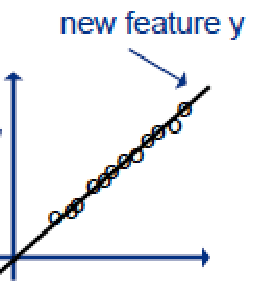
\includegraphics[width=0.3\linewidth]{figures/dimred2.pdf}
\end{center}

\alert{Principal component analysis} looks for a $d'$-dimensional linear subspace such that the projection of data points onto this subspace provides a ``faithful'' representation of the original dataset. By ``faithful'' representation, we mean that distances between original points and their projections are small—ideally minimal among all possible $d'$-dimensional subspaces. Equivalently, PCA seeks directions along which the projected data exhibits maximum variance, under the constraint that these directions are orthogonal to each other.

These equivalent perspectives provide both geometric intuition and computational algorithms for finding the optimal low-dimensional representation. As we will see, the solution involves computing the eigendecomposition of the sample covariance matrix $\displaystyle\mathbf{C} = \frac{1}{n}\mathbf{X}^T\mathbf{X}$, where the principal components are the eigenvectors corresponding to the largest eigenvalues, and the amount of variance explained by each component is given by its eigenvalue.


\subsubsection*{PCA for 0 dimension: Finding the Optimal Point}
Objective: represent all $d$-dimensional vectors $\x_{1},\ldots,\x_{n}$ by means of a unique vector $\x_{0}$, in the most faithful way, that is so that
\[
J(\x_{0})=\sum_{i=1}^{n}\vnorm{\x_{0}-\x_{i}}^{2}
\]
is minimum. It is easy to show that
\[
\x_{0}=\mathbf{m}=\frac{1}{n}\sum_{i=1}^{n}\x_{i}
\]
In fact, 

\begin{align*}
J(\x_{0})&=\sum_{i=1}^{n}\vnorm{(\x_{0}-\mathbf{m})-(\x_{i}-\mathbf{m})}^{2}=\sum_{i=1}^{n}\vnorm{\x_{0}-\mathbf{m}}^{2}+\sum_{i=1}^{n}\vnorm{\x_{i}-\mathbf{m}}^{2}
\end{align*}

Since
\[
\sum_{i=1}^{n}(\x_{i}-\mathbf{m})=\sum_{i=1}^{n}\x_{i}-n\cdot\mathbf{m}=n\cdot\mathbf{m}-n\cdot\mathbf{m}=0
\]
the second term is independent from $\x_{0}$, while the first one is equal to zero for $\x_{0}=\mathbf{m}$


\subsubsection*{PCA for One Dimension: Finding the Optimal Line}

This is the simplest nontrivial case: projecting data onto a one-dimensional subspace (a line). While projecting all data points to a single vector (the mean $\mathbf{m}$) is too extreme—losing all information about data variability—projecting onto a line through the mean provides a meaningful one-dimensional summary that preserves the direction of greatest variation.

\begin{center}
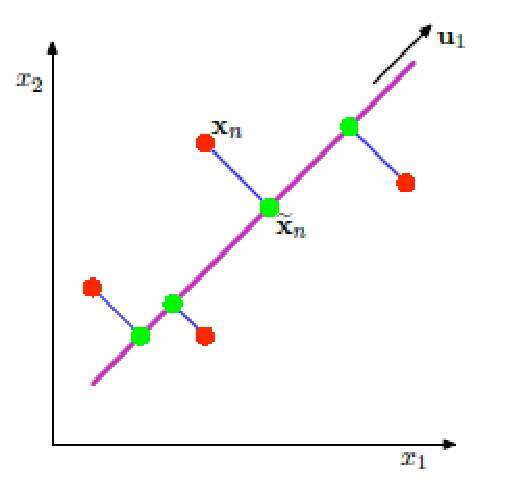
\includegraphics[width=0.4\linewidth]{figure/fig28.pdf}
\end{center}

\paragraph{Setting Up the Problem}

Let $\mathbf{u}_{1}$ be a unit vector ($\|\mathbf{u}_{1}\|=1$) specifying the direction of the line. Any point on this line passing through the mean $\mathbf{m}$ can be written as:
$$
\mathbf{x}=\alpha\mathbf{u}_{1}+\mathbf{m}
$$
where $\alpha$ represents the signed distance from $\mathbf{m}$ along the direction $\mathbf{u}_{1}$. For each data point $\mathbf{x}_{i}$ ($i=1,\ldots, n$), its projection onto the line is:
$$
\tilde{\mathbf{x}}_{i}=\alpha_{i}\mathbf{u}_1+\mathbf{m}
$$

Our goal is to find both the optimal projection coefficients $\{\alpha_i\}_{i=1}^n$ and the optimal direction $\mathbf{u}_1$ that together minimize the total reconstruction error—the sum of squared distances between original points and their projections:

\begin{align*}
J(\alpha_{1},\ldots,\alpha_{n},\mathbf{u}_{1})&=\sum_{i=1}^{n}\|\tilde{\mathbf{x}}_{i}-\mathbf{x}_{i}\|^{2}=\sum_{i=1}^{n}\|(\mathbf{m}+\alpha_{i}\mathbf{u}_{1})-\mathbf{x}_{i}\|^{2}
\end{align*}

Expanding this expression by using $\|\mathbf{a} - \mathbf{b}\|^2 = \|\mathbf{a}\|^2 + \|\mathbf{b}\|^2 - 2\mathbf{a}^T\mathbf{b}$ and noting that $\|\mathbf{u}_1\|^2 = 1$:
\begin{align*}
J(\alpha_{1},\ldots,\alpha_{n},\mathbf{u}_{1})&=\sum_{i=1}^{n}\|\alpha_{i}\mathbf{u}_{1} - (\mathbf{x}_{i}-\mathbf{m})\|^{2}\\
&=\sum_{i=1}^{n}\alpha_{i}^{2}+\sum_{i=1}^{n}\|\mathbf{x}_{i}-\mathbf{m}\|^{2}-2\sum_{i=1}^{n}\alpha_{i}\mathbf{u}_{1}^{T}(\mathbf{x}_{i}-\mathbf{m})
\end{align*}

To minimize $J$ with respect to each projection coefficient $\alpha_k$, we compute the partial derivative:
$$
\frac{\partial J}{\partial \alpha_{k}}=2\alpha_{k}-2\mathbf{u}_{1}^{T}(\mathbf{x}_{k}-\mathbf{m})
$$

Setting this equal to zero yields:
$$
\alpha_{k}=\mathbf{u}_{1}^{T}(\mathbf{x}_{k}-\mathbf{m})
$$

This is precisely the \alert{orthogonal projection} of the centered data point $\mathbf{x}_k - \mathbf{m}$ onto the direction $\mathbf{u}_1$—exactly what geometric intuition suggests. The second derivative confirms this is a minimum:
$$
\frac{\partial^2 J}{\partial \alpha_{k}^{2}}=2 > 0
$$

\paragraph{Finding the Optimal Direction}

Having determined the optimal projection coefficients in terms of $\mathbf{u}_1$, we now seek the direction that minimizes the reconstruction error. Substituting $\alpha_{i}=\mathbf{u}_{1}^{T}(\mathbf{x}_{i}-\mathbf{m})$ back into the error function:
\begin{align*}
J(\mathbf{u}_{1})&=\sum_{i=1}^{n}\alpha_{i}^{2}+\sum_{i=1}^{n}\|\mathbf{x}_{i}-\mathbf{m}\|^{2}-2\sum_{i=1}^{n}\alpha_{i}^{2}\\
&=-\sum_{i=1}^{n}\alpha_{i}^{2}+\sum_{i=1}^{n}\|\mathbf{x}_{i}-\mathbf{m}\|^{2}\\
&=-\sum_{i=1}^{n}[\mathbf{u}_{1}^{T}(\mathbf{x}_{i}-\mathbf{m})]^{2}+\sum_{i=1}^{n}\|\mathbf{x}_{i}-\mathbf{m}\|^{2}
\end{align*}

To connect this to the data covariance structure, we introduce the \alert{sample covariance matrix}:
$$
\mathbf{S}=\frac{1}{n}\sum_{i=1}^{n}(\mathbf{x}_{i}-\mathbf{m})(\mathbf{x}_{i}-\mathbf{m})^{T}
$$

Note that $[\mathbf{u}_{1}^{T}(\mathbf{x}_{i}-\mathbf{m})]^{2}$ can be rewritten using the identity $(a)(a)^T = a^2$ for scalars:
$$
[\mathbf{u}_{1}^{T}(\mathbf{x}_{i}-\mathbf{m})]^{2} = \mathbf{u}_{1}^{T}(\mathbf{x}_{i}-\mathbf{m})(\mathbf{x}_{i}-\mathbf{m})^{T}\mathbf{u}_{1}
$$

Summing over all data points:
$$
\sum_{i=1}^{n}\mathbf{u}_{1}^{T}(\mathbf{x}_{i}-\mathbf{m})(\mathbf{x}_{i}-\mathbf{m})^{T}\mathbf{u}_{1}=\mathbf{u}_{1}^{T}\left[\sum_{i=1}^{n}(\mathbf{x}_{i}-\mathbf{m})(\mathbf{x}_{i}-\mathbf{m})^{T}\right]\mathbf{u}_{1}=n\mathbf{u}_{1}^{T}\mathbf{S}\mathbf{u}_{1}
$$

Therefore, the reconstruction error becomes:
$$
J(\mathbf{u}_{1})=-n\mathbf{u}_{1}^{T}\mathbf{S}\mathbf{u}_{1}+\sum_{i=1}^{n}\|\mathbf{x}_{i}-\mathbf{m}\|^{2}
$$

\paragraph{Geometric Interpretation}

The term $\mathbf{u}_{1}^{T}\mathbf{S}\mathbf{u}_{1}$ has a natural interpretation: it represents the \alert{variance of the projected data} along direction $\mathbf{u}_1$. To see this, observe that:
\begin{itemize}
\item $\mathbf{u}_{1}^{T}(\mathbf{x}_{i}-\mathbf{m})$ is the projection of centered point $\mathbf{x}_i - \mathbf{m}$ onto $\mathbf{u}_1$
\item $[\mathbf{u}_{1}^{T}(\mathbf{x}_{i}-\mathbf{m})]^2$ is the squared distance of this projection from the origin
\item $\frac{1}{n}\sum_{i=1}^{n}[\mathbf{u}_{1}^{T}(\mathbf{x}_{i}-\mathbf{m})]^2 = \mathbf{u}_{1}^{T}\mathbf{S}\mathbf{u}_{1}$ is the variance of these projected values
\end{itemize}

Since the second term in $J(\mathbf{u}_1)$ is constant (independent of $\mathbf{u}_1$), minimizing the reconstruction error is \alert{equivalent to maximizing the variance of the projected data}:
$$
\min{\mathbf{u}_1} J(\mathbf{u}_{1}) \quad \Leftrightarrow \quad \max{\mathbf{u}_1} \mathbf{u}_{1}^{T}\mathbf{S}\mathbf{u}_{1}
$$

This reveals a fundamental principle of PCA: the direction that minimizes reconstruction error is precisely the direction along which the data exhibits maximum variance. Projecting onto this direction preserves as much information as possible in a single dimension.

\paragraph{Constrained Optimization via Lagrange Multipliers}

We seek to maximize $\mathbf{u}_{1}^{T}\mathbf{S}\mathbf{u}_{1}$ subject to the constraint $\|\mathbf{u}_{1}\|^2 = \mathbf{u}_{1}^{T}\mathbf{u}_{1}=1$ (ensuring $\mathbf{u}_1$ is a unit vector). Using the method of Lagrange multipliers, we form the Lagrangian:
$$
\mathcal{L}(\mathbf{u}_1, \lambda_1)=\mathbf{u}_{1}^{T}\mathbf{S}\mathbf{u}_{1}-\lambda_{1}(\mathbf{u}_{1}^{T}\mathbf{u}_{1}-1)
$$

Taking the derivative with respect to $\mathbf{u}_{1}$ and setting it to zero:
$$
\frac{\partial \mathcal{L}}{\partial \mathbf{u}_{1}}=2\mathbf{S}\mathbf{u}_{1}-2\lambda_{1}\mathbf{u}_{1}=\mathbf{0}
$$

This yields the \alert{eigenvalue equation}:
$$
\mathbf{S}\mathbf{u}_{1}=\lambda_{1}\mathbf{u}_{1}
$$

This reveals that the optimal direction $\mathbf{u}_{1}$ must be an \alert{eigenvector of the covariance matrix} $\mathbf{S}$.

\paragraph{Selecting the Principal Component}

To determine which eigenvector maximizes the variance, we substitute the eigenvalue equation into our objective:
$$
\mathbf{u}_{1}^{T}\mathbf{S}\mathbf{u}_{1}=\mathbf{u}_{1}^{T}(\lambda_{1}\mathbf{u}_{1})=\lambda_{1}\mathbf{u}_{1}^{T}\mathbf{u}_{1}=\lambda_{1}
$$

The variance of the projected data equals the eigenvalue $\lambda_1$. Therefore, to maximize this variance (and equivalently minimize reconstruction error), we must choose $\mathbf{u}_{1}$ to be the eigenvector corresponding to the \alert{largest eigenvalue} of $\mathbf{S}$. This eigenvector is called the \alert{first principal component}.

\paragraph{Extension to Higher Dimensions}

This analysis generalizes naturally to projections onto $d'$-dimensional subspaces with $d' > 1$. The optimal $d'$-dimensional subspace is spanned by the eigenvectors corresponding to the $d'$ largest eigenvalues of the covariance matrix $\mathbf{S}$. These eigenvectors, called \alert{principal components}, are mutually orthogonal and ordered by the amount of variance they explain:
$$
\lambda_1 \geq \lambda_2 \geq \cdots \geq \lambda_{d'} \geq \cdots \geq \lambda_d \geq 0
$$

\subsubsection*{An example of PCA}
Digit recognition ($D=28\times 28=784$)

\centerline{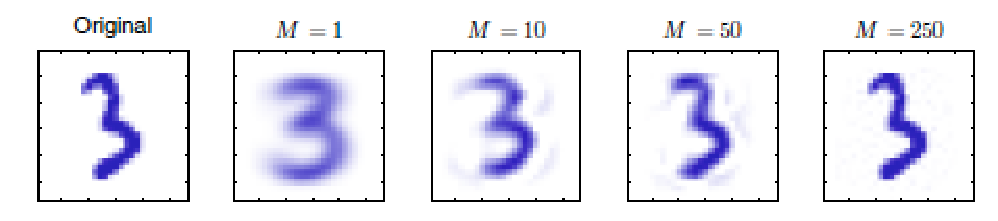
\includegraphics[width=0.4\linewidth]{figure/fig29.pdf}}


\subsubsection*{Choosing $d'$}
Eigenvalue size distribution is usually characterized by a fast initial decrease followed by a small decrease

\centerline{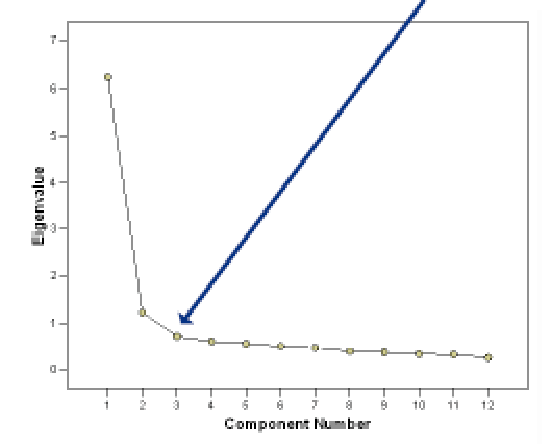
\includegraphics[width=0.4\linewidth]{figures/eigenpca.pdf}}

\medskip
This makes it possible to identify the number of eigenvalues to keep, and thus the dimensionality of the projections. 
Eigenvalues measure the amount of distribution variance kept in the projection.

\medskip
Let us consider, for each $k<d$, the value
\[
r_k=\frac{\sum_{i=1}^{k}\lambda_{i}^{2}}{\sum_{i=1}^{n}\lambda_{i}^{2}}
\]
which provides a measure of the variance fraction associated to the $k$ largest eigenvalues.

\medskip
When $r_{1}<\ldots<r_{d}$ are known, a certain amount $p$ of variance can be kept by setting 
\[
d'=\argmin{i\in\{1,\ldots,d\}}{r_{i}>p}
\] 



\subsection*{Fisher Linear Discriminant}

\subsubsection*{Motivation and Overview}

\emph{Linear Discriminant Analysis} (\emph{LDA}) is a supervised dimensionality reduction technique that seeks to find a linear projection of high-dimensional data into a lower-dimensional subspace where class separation is maximized. Unlike unsupervised methods such as PCA, which maximize variance without regard to class labels, LDA explicitly uses class information to find projections that make classification easier.

The \alert{Fisher linear discriminant} provides an elegant solution to this problem. In its simplest form, Fisher's approach projects $D$-dimensional data points onto a one-dimensional line via a linear transformation:
\begin{myequation}
y=\w\cdot \x=\w^{T}\x
\end{myequation}
where $\w$ is a $D$-dimensional weight vector that defines the direction of projection (normalized to unit length: $\|\w\|_2=1$).

\subsubsection*{Classification Rule}

For binary classification ($K=2$), the decision rule is straightforward: given a threshold $\tilde y$, an item $\x$ is assigned to class $C_{1}$ if its projection $y=\w^{T}\x$ satisfies $y>\tilde y$; otherwise, it is assigned to $C_{2}$.

\medskip
\centerline{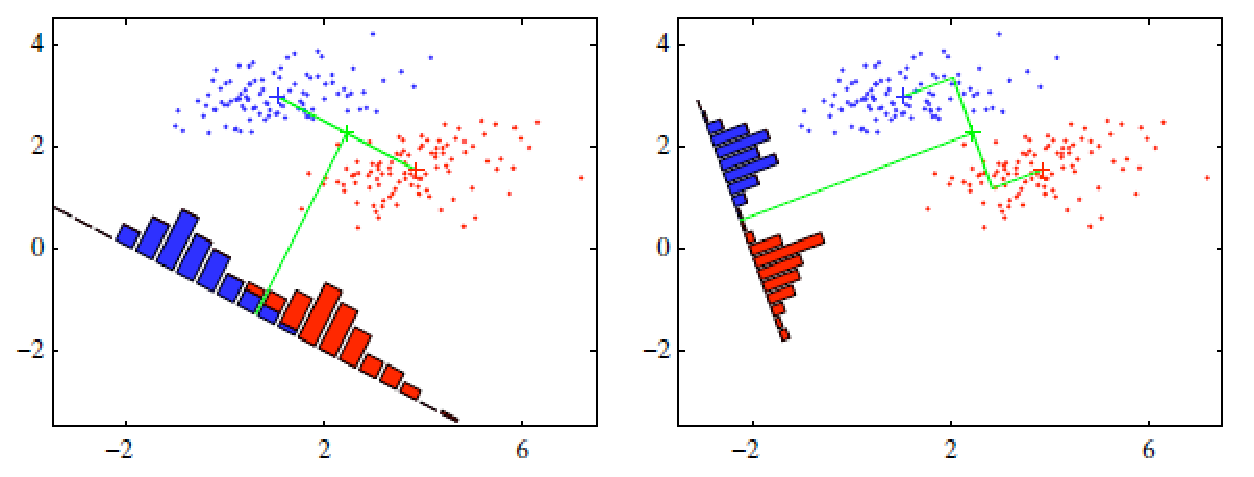
\includegraphics[width=0.5\linewidth]{figures/fisher.pdf}}

The choice of projection direction $\w$ is critical: different directions induce dramatically different class separability properties, as illustrated below.

\centerline{\begin{tabular}{rcl}
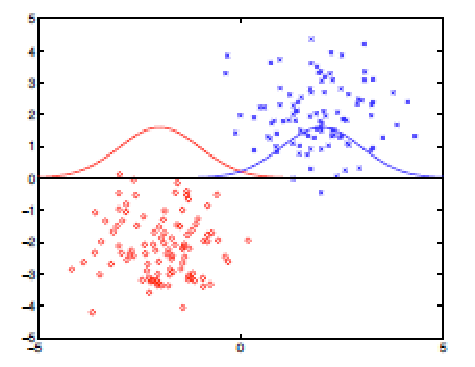
\includegraphics[width=0.3\textwidth]{figures/fisher21.pdf}&
 \hspace{2mm}&
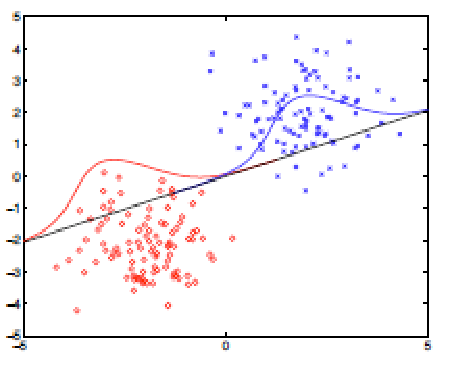
\includegraphics[width=0.3\textwidth]{figures/fisher22.pdf}\\
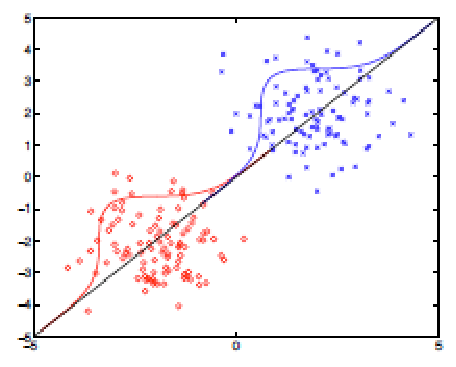
\includegraphics[width=0.3\textwidth]{figures/fisher23.pdf}&
 \hspace{2mm}&
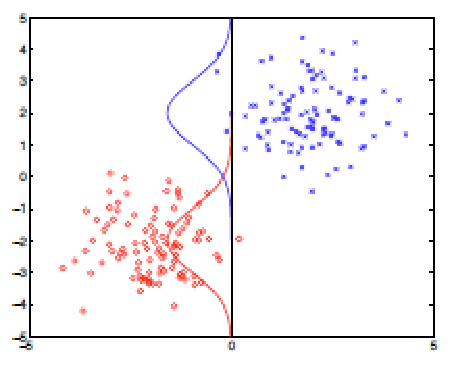
\includegraphics[width=0.3\textwidth]{figures/fisher24.pdf}
\end{tabular}}

\subsubsection*{Deriving the Optimal Direction $\w$}

\paragraph{First Attempt: Maximizing Class Mean Separation}

Let $n_{1}$ and $n_{2}$ denote the number of training samples in classes $C_{1}$ and $C_{2}$, respectively. The class mean vectors in the original $D$-dimensional space are:
\begin{myequation}
\mathbf{m}_{1}=\frac{1}{n_{1}}\sum_{\x\in C_{1}}\x\hspace{2cm}\mathbf{m}_{2}=\frac{1}{n_{2}}\sum_{\x\in C_{2}}\x
\end{myequation}

A natural measure of class separation after projection is the distance between the projected class means:
\begin{myequation}
m_{2}-m_{1}=\w^{T}(\mathbf{m}_{2}-\mathbf{m}_{1})
\end{myequation}
where $m_{i}=\w^{T}\mathbf{m}_{i}$ is the mean of class $C_i$ in the projected space.

To find the optimal direction:

\begin{itemize}
\item We want to maximize $m_{2}-m_{1}=\w^{T}(\mathbf{m}_{2}-\mathbf{m}_{1})$

\item However, this quantity can be made arbitrarily large by scaling $\w$. To ensure a well-defined solution, we constrain $\w$ to be a unit vector: $\|\w\|_{2}^2=\w^{T}\w=1$

\item This leads to the constrained optimization problem:
\begin{myalign}
&\max{\w}\w^{T}(\mathbf{m}_{2}-\mathbf{m}_{1})\\
&\text{subject to }\w^{T}\w=1
\end{myalign}

\item Using the method of \alert{Lagrange multipliers}, we convert this to an unconstrained problem:
\begin{myequation}
\max{\w,\lambda}\w^{T}(\mathbf{m}_{2}-\mathbf{m}_{1})+\lambda(1-\w^{T}\w)
\end{myequation}
\end{itemize}

Setting the gradient with respect to $\w$ to zero:
\begin{myequation}
\nabla_{\w} \left[\w^{T}(\mathbf{m}_{2}-\mathbf{m}_{1})+\lambda(1-\w^{T}\w)\right]=\mathbf{m}_{2}-\mathbf{m}_{1}-2\lambda\w=\Zero
\end{myequation}
yields:
\begin{myequation}
\w=\frac{\mathbf{m}_{2}-\mathbf{m}_{1}}{2\lambda}
\end{myequation}

Setting the derivative with respect to $\lambda$ to zero and applying the constraint $\w^{T}\w=1$:
\begin{myequation}\light{
\frac{\partial}{\partial\lambda}\left[\w^{T}(\mathbf{m}_{2}-\mathbf{m}_{1})+\lambda(1-\w^{T}\w)\right]=1-\w^{T}\w=0}
\end{myequation}
we obtain:
\begin{myequation}
\lambda=\frac{\|\mathbf{m}_{2}-\mathbf{m}_{1}\|_{2}}{2}
\end{myequation}

Combining these results:
\begin{myequation}
\w=\frac{\mathbf{m}_{2}-\mathbf{m}_{1}}{\|\mathbf{m}_{2}-\mathbf{m}_{1}\|_{2}}
\end{myequation}

This solution points from $\mathbf{m}_{1}$ toward $\mathbf{m}_{2}$.

\paragraph{Limitation of Mean Separation Alone}

Unfortunately, maximizing only the separation of class means often yields poor classification performance:

\medskip
\centerline{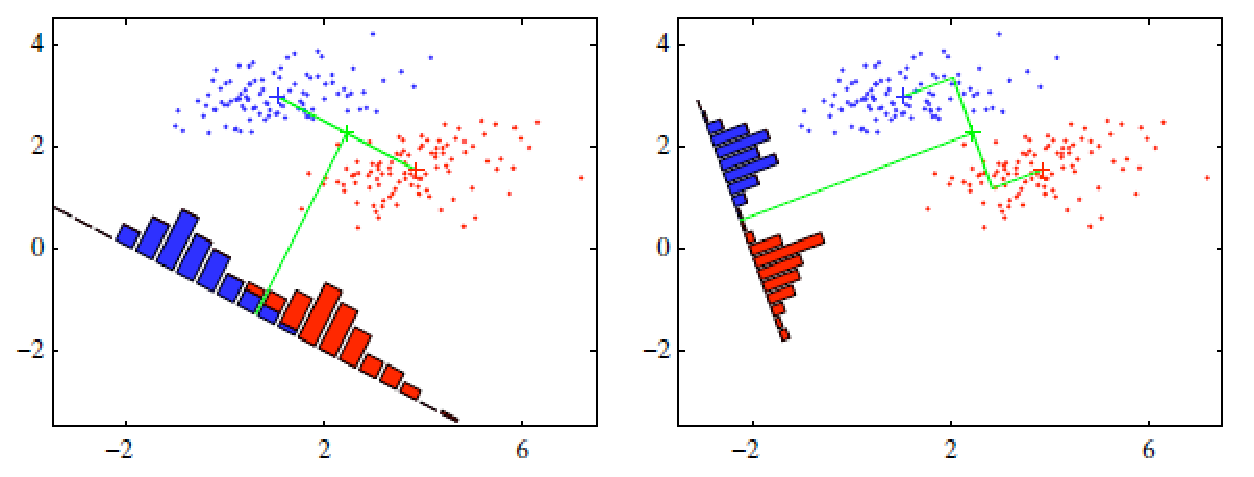
\includegraphics[width=0.7\textwidth]{figures/fisher.pdf}}

As shown above, projections along the direction $\mathbf{m}_2-\mathbf{m}_1$ can result in high within-class variance (dispersion), causing substantial overlap between classes even when their means are well separated.

\paragraph{Fisher's Solution: Accounting for Within-Class Variance}

Fisher's key insight was to balance two competing objectives:
\begin{itemize}
\item \textbf{Maximize} the separation between projected class means
\item \textbf{Minimize} the scatter (variance) of projections within each class
\end{itemize}

This approach is particularly effective when class distributions are elongated (anisotropic), so that different projection directions yield different amounts of within-class scatter.

Define the \alert{within-class variance} of the projection for class $C_{i}$ ($i=1,2$) as:
\begin{myequation}
s_{i}^{2}=\sum_{\x\in C_{i}}(\w^{T}\x-m_{i})^{2}
\end{myequation}

The \alert{Fisher criterion} is then defined as the ratio of between-class separation (squared) to total within-class variance:
\begin{myequation}
J(\w)=\frac{(m_{2}-m_{1})^{2}}{s_{1}^{2}+s_{2}^{2}}
\end{myequation}

This criterion increases with class separation and decreases with within-class scatter, precisely capturing our desiderata.

\paragraph{Matrix Formulation}

To derive the optimal $\w$ analytically, we introduce several covariance matrices. The \alert{within-class covariance matrix} for class $C_i$ is:
\begin{myequation}
\S_{i}=\sum_{\x\in C_{i}}(\x-\mathbf{m}_{i})(\x-\mathbf{m}_{i})^{T}
\end{myequation}

Using this definition, the within-class variance in the projected space can be written compactly as:
\begin{myequation}
s_{i}^{2}=\w^{T}\S_{i}\w
\end{myequation}

Define the \alert{total within-class covariance matrix} as $\S_W=\S_1+\S_2$, and the \alert{between-class covariance matrix} as:
\begin{myequation}
\S_{B}=(\mathbf{m}_{2}-\mathbf{m}_{1})(\mathbf{m}_{2}-\mathbf{m}_{1})^{T}
\end{myequation}

The Fisher criterion can now be expressed in matrix form:
\begin{myequation}
J(\w)=\frac{(m_{2}-m_{1})^{2}}{s_{1}^{2}+s_{2}^{2}}=\frac{\w^{T}\S_{B}\w}{\w^{T}\S_{W}\w}
\end{myequation}

\paragraph{Optimization}

To maximize $J(\w)$, we set its gradient to zero:
\begin{myequation}
\nabla_{\w} \frac{\w^{T}\S_{B}\w}{\w^{T}\S_{W}\w}=\Zero
\end{myequation}

%\begin{lightblock}
Applying the quotient rule for gradients yields:
\begin{myequation}
(\w^{T}\S_B\w)\S_W\w-(\w^{T}\S_W\w)\S_B\w=\Zero
\end{myequation}
which simplifies to:
\begin{myequation}
(\w^{T}\S_B\w)\S_W\w=(\w^{T}\S_W\w)\S_B\w
\end{myequation}
%\end{lightblock}

%\begin{lightblock}
Note that:
\begin{itemize}
  \item $\w^T\S_B\w$ is a scalar (say $c_B$)
  \item $\w^T\S_W\w$ is a scalar (say $c_W$)
  \item Since $\S_B=(\mathbf{m}_2-\mathbf{m}_1)(\mathbf{m}_2-\mathbf{m}_1)^T$, we have $\S_B\w=(\mathbf{m}_2-\mathbf{m}_1)c_m$ where $c_m=(\mathbf{m}_2-\mathbf{m}_1)^T\w$ is a scalar
\end{itemize}

Substituting into the optimality condition:
\begin{myequation}
c_B\S_W\w=c_W(\mathbf{m}_2-\mathbf{m}_1)c_m
\end{myequation}

Solving for $\w$:
\begin{myequation}
\w=\frac{c_Wc_m}{c_B}\S_W^{-1}(\mathbf{m}_2-\mathbf{m}_1)
\end{myequation}
%\end{lightblock}

Since we are only interested in the \emph{direction} of $\w$ (any positive scalar multiple defines the same projection direction), we obtain the \alert{Fisher's linear discriminant solution}:
\begin{myequation}
\hat{\w}=\S_W^{-1}(\mathbf{m}_2-\mathbf{m}_1)=(\S_1+\S_2)^{-1}(\mathbf{m}_2-\mathbf{m}_1)
\end{myequation}

This elegant result shows that the optimal direction is obtained by first computing the vector connecting the class means, then transforming it by the inverse of the pooled within-class covariance matrix.

\subsubsection*{Choosing the Classification Threshold}

Once the projection direction $\hat{\w}$ is determined, we need to select a threshold $\tilde{y}$ for classification. A principled approach based on probabilistic modeling:

\begin{itemize}
  \item Model the projected data for each class as Gaussian: $p(y|C_i)\sim\mathcal{N}(m_i, \sigma_i^2)$
  
  \item Estimate parameters via maximum likelihood:
  \begin{myequation}
  m_i=\frac{1}{n_i}\sum_{\x\in C_i}\w^T\x\hspace{1cm}\sigma_i^2=\frac{1}{n_i-1}\sum_{\x\in C_i}(\w^T\x-m_i)^2
  \end{myequation}
  where $n_i$ is the number of training samples in class $C_i$
  
  \item Apply Bayes' rule to compute posterior probabilities:
  \begin{myequation}
  p(C_i|y)\propto p(y|C_i)p(C_i)=p(y|C_i)\frac{n_i}{n_1+n_2}\propto n_i\exp\left(-\frac{(y-m_i)^2}{2\sigma_i^2}\right)
  \end{myequation}
  
\item The decision threshold $\tilde{y}$ is the value where the class posteriors are equal. Equivalently, choose $\tilde{y}$ as the smallest $y$ satisfying:
\begin{myequation}
\frac{p(C_2|y)}{p(C_1|y)}=\frac{n_2}{n_1}\frac{p(y|C_2)}{p(y|C_1)}>1
\end{myequation}
\end{itemize}

This threshold balances the trade-off between false positives and false negatives, taking into account both the class-conditional distributions and prior class probabilities.

\subsection*{Autoencoders}

Autoencoders project features on a smaller space by applying a non linear transformation implemented by a neural network. Indeed an autoencoder encodees the input into a compressed and meaningful representation, and then decode it back such that the reconstructed input is similar as possible to the original one. Their main purpose is learning in an unsupervised manner an ``informative'' representation of the data that can be used for various implications such as clustering. 

Formally, an $n/p/n$ autoencoder can be defined  in terms of
\begin{itemize}
\item a class of \alert{encoder} functions $\mathcal{E}$, from $\mathbb{R}^n$ to $\mathbb{R}^p$ 
\item a class of \alert{decoder} functions $\mathcal{D}$, from $\mathbb{R}^p$ to $\mathbb{R}^n$
\item a \alert{reconstruction loss} function $\mL: \mathbb{R}^n\times \mathbb{R}^n\mapsto \mathbb{R}$
\end{itemize}
The problem is finding a pair of encoder and decoder functions $e^*\in \mathcal{E}$, $d^*\in\mathcal{D}$ such that
\begin{myequation}
(e^*,d^*) = \argmin{e\in\mathcal{E},d\in\mathcal{D}}\med{\x}{\mL(\x, d(e(\x)))}
\end{myequation}
that is, we are interested in finding the encode-decoder pair which minimizes the (expected) difference between the input $\x$ and the result of the sequence of encoding and decoding $d(e(\x))$. The reconstruction loss is usually set to be the $\ell_2$-norm, that is $\mL(\x,\y)=||\x-\y||^2=\sum_{i=1}^n{(x_i-y_i)}^2$.

Figure~\ref{fig:Autoencoder} provides an illustration of the autoencoder model.

\begin{figure}
\begin{center}
\begin{tikzpicture}
\Vertex[Math, x=0, y=0, color=xkcdTurquoise, opacity=.5, shape = rectangle, fontsize=\footnotesize, style={minimum width=.3cm, minimum height=2.5cm, line width=.1pt}]{B1}
\Text[x=0,y=1.5, distance=7mm, fontsize=\footnotesize]{$\x$}
\Text[position=left, x=0,y=.5, distance=2mm, fontsize=\scriptsize]{$n$}

\Vertex[Math, x=1.5,y=0, color=xkcdBuff, label = e, size = 1, opacity=.5, fontsize=\large, style={line width=.5pt}]{C}
 \Edge[lw=.5pt, Direct](B1)(C)
 
\Vertex[Math, x=3, y=0, color=xkcdLipstickRed, opacity=.5, shape = rectangle, fontsize=\footnotesize, style={minimum width=.3cm, minimum height=1.5cm, line width=.1pt}]{B2}
\Text[x=3,y=1.5, distance=7mm, fontsize=\footnotesize]{$\z=e(\x)$}
\Text[position=left, x=3,y=.5, distance=2mm, fontsize=\scriptsize]{$p$}

 \Edge[lw=.5pt, Direct](C)(B2)
 
 \Vertex[Math, x=4.5,y=0, color=xkcdBurntOrange, label = d, size = 1, opacity=.5, fontsize=\large, style={line width=.5pt}]{C1}
 \Edge[lw=.5pt, Direct](B2)(C1)
 
 \Vertex[Math, x=6, y=0, color=xkcdFadedBlue, opacity=.5, shape = rectangle, fontsize=\footnotesize, style={minimum width=.3cm, minimum height=2.5cm, line width=.1pt}]{B3}
 \Text[x=6,y=1.5, distance=7mm, fontsize=\footnotesize]{$\y=d(\z)$}
\Text[position=right, x=6,y=.5, distance=2mm, fontsize=\scriptsize]{$n$}
 \Edge[lw=.5pt, Direct](C1)(B3)
 
  \Edge[lw=.5pt, bend=90, label=loss, fontsize=\small, style={dashed,color=xkcdRed}](B1)(B3)
\end{tikzpicture}
\end{center}
\caption{General structure of an autoencoder.}%
\label{fig:Autoencoder}
\end{figure}


\begin{figure}
\begin{center}
\resizebox{0.8\textwidth}{!}{%
\begin{tikzpicture}[
    shorten >=1pt, shorten <=1pt, >=stealth',
    neuron/.style={circle, draw, minimum size=4ex, thick, fill=#1, opacity=0.7},
    legend/.style={font=\large\bfseries},
  ]

  % encoder
  \drawNodes{encoder}{{{,,,,,}, {,,,,}, {,,,,}}}{xkcdTeal}
  \denselyConnectNodes{encoder}{{6, 5, 5}}

  % decoder
  \begin{scope}[xshift=7cm]
    \drawNodes{decoder}{{{,,,}, {,,,,,}}}{xkcdBuff}
    \denselyConnectNodes{decoder}{{4, 6}}
  \end{scope}

  % mu, sigma, sample nodes
  \foreach \idx in {1,...,3} {
      \coordinate[neuron, right=1 of encoder-3-3, yshift=\idx cm-2cm, fill=xkcdFadedBlue, fill opacity=0.7] (latent-\idx);
    }

 % mu, sigma, sample boxes
 \node [label=latent, fit=(latent-1) (latent-3), draw, fill=xkcdFadedBlue, opacity=0.2] (latent) {};
 \node [label=Encoder, fit=(encoder-1-1) (encoder-3-5) (encoder-1-6), draw, fill=xkcdTurquoise, opacity=0.2] (encoder) {};
 \node [label=Decoder, fit=(decoder-1-1) (decoder-2-1) (decoder-2-6), draw, fill=xkcdBuff, opacity=0.2] (decoder) {};
   
  % mu, sigma, sample connections
 % \draw[->] (mu.east) edge (sample.west) (sigma.east) -- (sample.west);
  \foreach \a in {1,2,3,4,5}
  \foreach \b in {1,2,3} {
      \draw[->] (encoder-3-\a) -- (latent-\b);
    }
    
  \foreach \a in {1,2,3,4}
  \foreach \b in {1,2,3} {
      \draw[->] (latent-\b) -- (decoder-1-\a);
    }

  % input + output labels
  \foreach \idx in {1,...,6} {
      \node[left=0.2 of encoder-1-\idx] {$x_\idx$};
      \node[right=0.2 of decoder-2-\idx] {$\hat x_\idx$};
    }
  \node[above left=0.5 of encoder-1-4] {input};
  \node[above right=0.5 of decoder-2-4] {output};

\end{tikzpicture}
    }%
\end{center}
\caption{Neural network implementation of an autoencoder.}%
\label{fig:Autoencoder_nn}
    %\label{fig:var_encoder}
\end{figure}



As we may see, starting from $\x$, the encoder derives a new vector $\z$ of a different (usually smaller) size: this is called a \alert{latent representation} of $\x$
In the most popular form of autoencoders, $e$ and $d$ are implemented by neural networks.

In the special case that $\mathcal{E}$ and $\mathcal{D}$ are classes of linear operations, we get a linear autoencoder: in this case, each component of $\z$ is a linear combination of components of $\x$, and each component of $\y$ is a linear combination of components of $\z$. In the case of a linear autoencoder the same latent representation as Principal Component Analysis (PCA) is achieved. Therefore, an autoencoder is in fact a generalization of PCA, where instead of finding a low dimensional hyperplane in which the data lies, it is able to learn a non-linear manifold. In addition, the autoencoder is explicitly optimized for the data reconstruction from the code. A good intermediate representation not only can capture latent variables, but also benefits a full decompression process.

As usual in Machine Learning, the set of functions to be considered are defined as classes of parametric functions with parameters $\Vtheta$ for the encoder and $\Vphi$ for the decoder. The loss function is then minimized wrt the encoder and the decoder parameters:
\begin{equation*}
(\Vtheta^*,\Vphi^*) = \argmin{\Vtheta,\Vphi}\med{\x}{\mL(\x, d(e(\x;\Vtheta), \Vphi))}
\end{equation*}
The parametric functions are usually implemented as neural networks.

\begin{figure}
\begin{center}
\begin{tikzpicture}
\Vertex[Math, x=1.25,y=0, color=xkcdTurquoise, opacity=.8, shape = rectangle, label = \x, fontsize=\footnotesize, style={minimum width=2cm, minimum height=3mm, line width=.1pt}]{B0}
  \Text[position=below,x=1.25,y=0, distance=1.2mm, fontsize=\scriptsize]{$n$}
  \Vertex[Math, x=3.5,y=0, color=xkcdBuff, opacity=.5, shape = rectangle, label = W_e, fontsize=\footnotesize, style={minimum width=1cm, minimum height=2cm, line width=.5pt}]{W1}
  \Text[position=above,x=3.5,y=0, distance=11mm, fontsize=\scriptsize]{$p$}
  \Text[position=right,x=3.5,y=.5, distance=6mm, fontsize=\scriptsize]{$n$}
  \Edge[lw=.5pt, Direct](B0)(W1)
  
  \Vertex[Math, x=4.75,y=0, color=xkcdLightGrey, label = +, size = .4, opacity=.5, fontsize=\footnotesize, style={line width=.5pt}]{C}
  \Edge[lw=.5pt, Direct](W1)(C)
  
\Vertex[Math, x=4.75,y=-1, color=xkcdBuff, label = b, opacity=.5, shape = rectangle, fontsize=\footnotesize, style={minimum width=9mm, minimum height=3mm, line width=.5pt}]{B3}
\Text[position=below,x=4.75,y=-1, distance=2mm, fontsize=\scriptsize]{$p$}
\Edge[lw=.5pt, Direct](B3)(C)
    
\Vertex[Math, x=6,y=0, color=xkcdLipstickRed, label=\z, opacity=.5, shape = rectangle, fontsize=\footnotesize, style={minimum width=1cm, minimum height=3mm, line width=.1pt}]{B2}
 \Text[position=below,x=6,y=0, distance=2mm, fontsize=\scriptsize]{$p$}
 \Edge[lw=.5pt, Direct](C)(B2)
  
\Vertex[Math, x=8,y=0, color=xkcdBurntOrange, opacity=.5, shape = rectangle, label = W_d, fontsize=\footnotesize, style={minimum width=2cm, minimum height=1cm, line width=.5pt}]{B4}
  \Text[position=above,x=8,y=0, distance=6mm, fontsize=\scriptsize]{$n$}
  \Text[position=right,x=8.5,y=.25, distance=5mm, fontsize=\scriptsize]{$p$}
\Edge[lw=.5pt, Direct](C1)(B2)
\Edge[lw=.5pt, Direct](B2)(B4)
  
\Vertex[Math, x=10,y=0, color=xkcdLightGrey, label = +, size = .4, opacity=.5, fontsize=\footnotesize, style={line width=.5pt}]{C2}
\Edge[lw=.5pt, Direct](B4)(C2)
  
\Vertex[Math, x=10,y=-1, color=xkcdBurntOrange, label = b', opacity=.5, shape = rectangle, fontsize=\footnotesize, style={minimum width=2cm, minimum height=3mm, line width=.5pt}]{B5}
\Text[position=below,x=10,y=-1, distance=2mm, fontsize=\scriptsize]{$n$}
\Edge[lw=.5pt, Direct](B5)(C2)
    
 \Vertex[Math, x=12,y=0, color=xkcdFadedBlue, label=\y, opacity=.5, shape = rectangle, fontsize=\footnotesize, style={minimum width=2cm, minimum height=3mm, line width=.1pt}]{C6}
 \Text[position=below,x=12,y=0, distance=2mm, fontsize=\scriptsize]{$n$}
\Edge[lw=.5pt, Direct](C2)(C6)
  \Edge[lw=.5pt, bend=90, label=loss, fontsize=\small, style={dashed,color=xkcdRed}](B0)(C6)
\end{tikzpicture}
\end{center}
\caption{Structure of a linear autoencoder.}%
\label{fig:lin_autoencoder}
\end{figure}
Adding a "bottleneck," (more on that later) is achieved by making the latent feature's dimensionality lower (often much lower) than the input's. That is the case that we will look in detail in this article. But before looking at this case, let’s briefly discuss regularization.

%\subsection{Regularized autoencoders}
%\label{sec:Regularized_autoencoders}
Since in training, one may just get the identity operator for $e$ and $d$, which keeps the achieved representation the same as the input, some additional regularization is required. The most common option is to make the dimension of the representation smaller than the input. This way, a \alert{bottleneck} is imposed. This option also directly serves the goal of getting a low dimensional representation of the data. This representation can be used for purposes such as data compression, feature extraction, etc. Its important to note that even if the bottleneck is comprised of only one node, then overfitting is still possible if the capacity of the encoder and the decoder is large enough to encode each sample to an index.

In cases where the size of the hidden layer is equal or greater than the size of the input, there is a risk that the encoder will simply learn the identity function. To prevent it without creating a bottleneck (i.e.\, smaller hidden layer) several options exists for regularization that would enforce the autoencoder to learn a different representation of the input.







%\end{document}